\documentclass{scrartcl}
\usepackage{etoolbox}
\usepackage{bbm}
\usepackage{amsmath}
\usepackage{mathabx}
\usepackage{graphicx}
\usepackage{float}
\usepackage{parskip}
\usepackage{indentfirst}
\usepackage{subfigure}
\setlength{\parskip}{0em}
\setlength{\parindent}{2em}

%-----------------------------------------------------------------------------
\begin{document}

%-----------------------------------------------------------------------------
% title
\title{\LARGE SoCal: Genotype Calling via Ellipsoidal Separation}
\author{\large Huwenbo Shi (603-778-363) shihuwenbo@ucla.edu}
\date{}
\maketitle
%-----------------------------------------------------------------------------


%-----------------------------------------------------------------------------
% abstract
\begin{abstract}
    \begin{center}
        ABSTRACT
    \end{center}
    
\par
In this article, I present SoCal, a supervised genotype calling algorithm for
Affymetrix SNP arrays.
For each SNP, SoCal first efficiently identify ellipsoidal decision regions for
each genotype from reference genotype calls, and then uses these regions to
classify future SNPs into different genotypes.
Using only a small portion of training genotype calls from the HapMap Project,
SoCal achieves an accuracy of $97.5\%$ during validation.
\end{abstract}
%-----------------------------------------------------------------------------


%-----------------------------------------------------------------------------
% introduction
\section{Introduction}

\par
Single nucleotide polymorphisms (SNPs), genomic positions at which a single
nucleotide differs between individuals, are responsible for many phenotypic
variations among individuals.
To study the associations between SNPs and phenotypes, one must be able to
accurately call genotypes for case and control samples at these SNPs.
Although next generation sequencing (NGS) technology provides cheap and
whole-genome sequences for genotyping SNPs, SNP arrays are still more
cost-effective for specific experiments \cite{rho2010}.

\par
Affymetrix SNP arrays use oligonucleotide probes to measure intensities
$I_A$ and $I_B$ for alleles $A$ and $B$ of SNPs in samples.
If a sample has genotype $AA$ or $BB$ for a SNP, one observes higher value of
$I_A$ or $I_B$ respectively.
For genotype $AB$, one observes similar values of $I_A$ and $I_B$.
If one plots the data point ($I_A$, $I_B$) of a SNP for a number of samples,
normally 3 clusters are observed, one for each genotype
(Figure \ref{fig:intro_genclus}).
The computational challenge is to correctly assign each ($I_A$, $I_B$)
data point to a cluster and call its genotype accordingly.

\par
Many genotype calling algorithms use model-based unsupervised clustering
methods to identify clusters and then assign genotypes to each cluster.
For instance, Norl\'{e}n et al. proposed a Gaussian mixture model for
clustering \cite{norlen2008}.
Lin et al. proposed a statistical model and a modified
K-means algorithm to incorporate pedigree information in clustering
\cite{lin2008}.
These methods use EM algorithm to estimate model parameters, which is sensitive
to starting parameters and slow to converge \cite{wu1983}.

\par
A few other genotype calling algorithms exploit reference genotype calls.
For instance, Rabbee et al. proposed the RLMM algorithm, which estimates allele
intensities of SNPs on a chip by fitting a linear mixed model and compares
them with the means obtained from training data to call genotypes
\cite{rabbee2005}. 
This method models probe effect in the linear mixed model and is able to make
more accurate genotype calls.
However, fitting a linear mixed model can be computationally intensive, and
may involve optimizing a non-convex function \cite{zhou2014}.

\par
As the number of probes on SNP arrays and the number of individuals involved
in association studies continue to increase, both fast and accurate genotype
calling algorithms are needed.
In this article, I developed a supervised genotype calling algorithm (SoCal)
that uses reference genotype calls from HapMap to efficiently find elliptic
boundaries separating the three genotypes from one another for each SNP.
SoCal then uses these boundaries to call the same SNP in different samples with
unknown genotypes in linear time.
SoCal can also control outlier effect by using different criteria for finding
the separating boundaries, a feature not provided by simply fitting a Gaussian
distribution.

\begin{figure}[H]
    \centering
    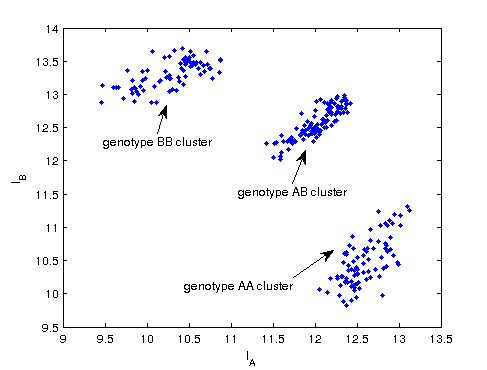
\includegraphics[scale=0.75]
    {introduction_figures/introductoin_cluster.png}
    \caption{Genotype clusters obtained from Affymetrix SNP array
             allele intensity values}
    \label{fig:intro_genclus}
\end{figure}
%-----------------------------------------------------------------------------


%-----------------------------------------------------------------------------
% method
\section{Method}

\par
SoCal calls genotypes in two steps.
The first step of SoCal is finding decision regions for each genotye
using reference genotype calls for a specific SNP.
The second step of SoCal is using these decision regions to
classify the same SNP into different genotypes for different samples.

\subsection{Finding decision regions}

\par
Affymetrix SNP arrays generate allele intensity values that roughly follow
bivariate Gaussian distributions.
Because of outliers in reference genotype calls, simply fitting bivariate
Gaussian distributions and then applying likelihood ratio test might not the
best way of classifying genotypes.
Instead, SoCal uses ellipses as decision regions, and controls outlier effect
by specifying different criteria for finding the ellipses.

\par
An ellipsoid $\mathcal{E} \subseteq \mathbbm{R}^{n}$ can be expressed as
$\mathcal{E} = \{x \in \mathbbm{R}^{n} | (x-c)^TE(x-c)\leqslant1\}$, where
$c$ is the center of the ellipsoid, and $E$ a positive semidefinite matrix.
Let $a_i$ be the points to be included in an ellipsoidal region, and $b_j$
be the points to be excluded, the problem is to find a $c$ and $E$ that
separate $a_i$ from $b_j$.

\par
For SoCal, the dimension of data is $2$ ($n=2$). $a_i$ correponds to the allele
intensity data points of one genotype, and $b_j$ correponds to the allele
intensity data points of all other genotypes. For each SNP, SoCal obtains
three $c$'s and three $E$'s, one for each genotype.

\par
In the following subsections, three different ways of finding elliptical
decision regions are discussed.

\subsubsection{Maximal separation ratio method (MAXSEP)}

\par
MAXSEP, discussed in detail in \cite{glineur1998},
tries to find ellipses that separate $a_i$ from $b_j$ with the maximum
separation ratio.
This problem can be expressed as a conic programming problem:
\begin{gather*}
\mathrm{minimize}\;-k \\
\mathrm{subject\;to}\;\;
(1,a_i)^T\tilde{E}(1,a_i)\leqslant1 \; \forall i \\
\;\;\;\;\;\;\;\;\;\;\;\;\;\;\;\;\;\;\;
(1,b_j)^T\tilde{E}(1,b_j) \ge k \; \forall j \\
\;\;\;\;\;\;\;\;\;\;\;\;\;\;\;\;\;\;\;
\tilde{E} \succeq 0.
\end{gather*}

\par
Let 
\begin{gather*}
    \tilde{E}^{*}=\left[
    \begin{array}{cc}
    s & v^T \\
    v & F
    \end{array}
    \right]
\end{gather*}
be the optimal solution to the problem above.
The maximum margin separating ellipsoid $\mathcal{E}^{*}$ is defined as
\begin{gather*}
\mathcal{E}^{*}=
\{x \in \mathbbm{R}^{n} | (x-c^{*})^TE^{*}(x-c^{*})\leqslant2(1+k)\},
\end{gather*}
where
\begin{gather*}
c^{*}=-F^{-1}v,\;E^{*}={{F} \over {(1-s+{c^{*}}^TF{c^{*}})}}.
\end{gather*}

\par
Intuitively, the first constraint in the problem formulation above forces the
ellipsoid to contain all the $a_i$ points.
The second constraint tries to find ellipses that separate $b_j$ from $a_i$
as much as possible.
The final result $c^{*}$ and $E^{*}$ separates $a_i$ and $b_j$ using an ellipse
with the largest margin.

\subsubsection{Minimum volume method (MINVOL)}

\par
MINVOL,discussed in detail in \cite{glineur1998},  tries to enclose a set of
points in an ellipsoid with minimum volume.
Finding a minimum volume enclosing ellipsoid can also be expressed as a conic
programming problem:
\begin{gather*}
    \mathrm{minimize}\;trace(T) \\
    \mathrm{subject\;to}\;\;
    (1,a_i)^T\tilde{E}(1,a_i)\leqslant1 \; \forall i \\
    \;\;\;\;\;\;\;\;\;\;\;\;\;\;\;\;\;\;\;
    \tilde{E}=
    \left[
        \begin{array}{cc}
            s & v^T \\
            v & F
        \end{array}
    \right] \succeq 0 \\
    \;\;\;\;\;\;\;\;\;\;\;\;\;\;\;\;\;\;\;
    \left[
        \begin{array}{cc}
            F & I \\
            I & T
        \end{array}
    \right] \succeq 0
\end{gather*}

\par
The minimum volume encolsing ellipsoid $\mathcal{E}^{*}$ is defined as
$\mathcal{E}^{*}=
\{x \in \mathbbm{R}^{n} | (x-c^{*})^TE^{*}(x-c^{*})\leqslant1\}$,
where
$c^{*}=-F^{-1}v$, $E^{*}=F/(1-s+{c^{*}}^TF{c^{*}})$.

\par
In the problem formulation above, $trace(T)$ models the volume of ellipsoid,
as it can be shown that
$boxsize(E)=\sqrt{\sum_{i=1}^n \lambda_{i}(E)^{-1}}$ approximates the volume
of a ellipsoid $E$ (Figure~\ref{fig:method_box}).
The constraint of the problem formulation in essence guarantees that
$T \succeq E^{-1}$, which can be derived by applying Schur complement.

\begin{figure}[H]
    \centering
    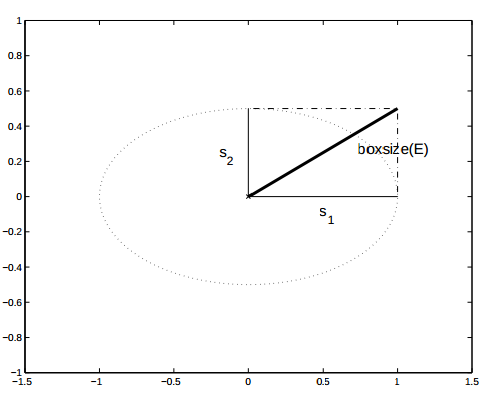
\includegraphics[scale=0.5]
    {method_figures/method_box.png}
    \caption{$boxsize$ approximation of ellipsoid volume, 
             adapted from \cite{glineur1998}}
    \label{fig:method_box}
\end{figure}

\subsubsection{Combined approach (COMB)}

\par
The previous two methods for finding separating ellipsoids always find
the ones that enclose all the points of one class.
However, because of outliers in dataset, not all data points should be
used - elliminating some data points during ellipsoid
construction may lead to better classification result.
For an extreme example, in Figure~\ref{fig:method_outlier}, if one tries
to separate the red points from the blue points using MINVOL, one will get the
outer ellipse as the decision region for the red points, which is obviously not
a good decision region.

\par
Instead, COMB provides a flexible way to control outlier effect using an
approach that combines the previous two methods with an additional $l_1$-norm
regularization.
The method of COMB can be expressed as a convex programming problem:
\begin{gather*}
    \mathrm{minimize}\;-{\beta_{1}}k+{\beta_{2}} trace(T)+\beta_{3} \|u-1\|_1 \\  
    \mathrm{subject\;to}\;\;
    (1,a_i)^T\tilde{E}(1,a_i)\leqslant u_i \; \forall i \\
    \;\;\;\;\;\;\;\;\;\;\;\;\;\;\;\;\;\;\;
    (1,b_j)^T\tilde{E}(1,b_j) \ge k \; \forall j \\
    \;\;\;\;\;\;\;\;\;\;\;\;\;\;\;\;\;\;\;
    \tilde{E}=
    \left[
        \begin{array}{cc}
            s & v^T \\
            v & F
        \end{array}
    \right] \succeq 0 \\
    \;\;\;\;\;\;\;\;\;\;\;\;\;\;\;\;\;\;\;
    \left[
        \begin{array}{cc}
            F & I \\
            I & T
        \end{array}
    \right] \succeq 0,
\end{gather*}
where $\beta_{i} > 0$ are the weights assigned to each sub-objectives:
maximizing separation ratio, minimizing ellipsoid volume, and controlling
outliers.
The final ellipsoidal decision region $\mathcal{E}^{*}$ is defined as
$\mathcal{E}^{*}=
\{x \in \mathbbm{R}^{n} | (x-c^{*})^TE^{*}(x-c^{*})\leqslant2(1+k)\}$,
where
$c^{*}=-F^{-1}v$, $E^{*}=F/(1-s+{c^{*}}^TF{c^{*}})$.

\par
In Figure~\ref{fig:method_outlier}, if one sets
$\beta_{1}=\beta_{2}=\beta_{3}=1$, one will get the inner ellipse as the
decision region for red points, which is clearly a much better decision region
than the outer ellipse obtained using MINVOL.

\begin{figure}[H]
    \centering
    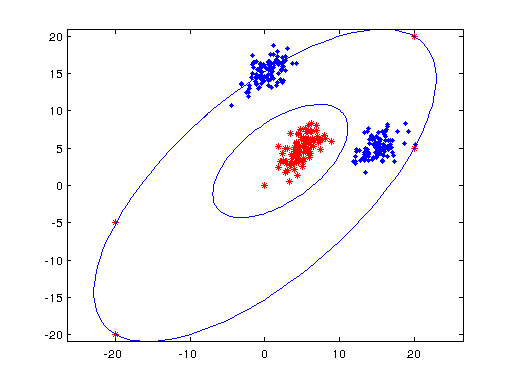
\includegraphics[scale=0.75]
    {method_figures/comb_outlier.png}
    \caption{COMB finds better ellipsoidal decision regions when there are
             outliers}
    \label{fig:method_outlier}
\end{figure}

\subsection{Classification}

\par
Once the elliptical decision regions,
$\mathcal{E}_{t}^{*}=
\{x \in \mathbbm{R}^{n} | (x-c_t^{*})^TE_t^{*}(x-c_t^{*})\leqslant1\}$, for
$t=AA,AB,BB$, for a specific SNP, are obtained, SoCal uses them to call
genotypes for samples with unknown genotype for the same SNP.

\par
For each sample with allele intensity $I_A$ and $I_B$, SoCal computes
\begin{gather*}
D_t=(y-c_t^{*})^TE_t^{*}(y-c_t^{*}),
\end{gather*}
where $y=(I_A,I_B)$, for $t=AA,AB,BB$.
SoCal then assigns genotype with the minimum $D_t$ to that sample, that is
\begin{gather*}
G=\operatorname*{arg\,min}_{t\in \{AA,AB,BB\}}
(y-c_t^{*})^TE_t^{*}(y-c_t^{*}).
\end{gather*}
%-----------------------------------------------------------------------------


%-----------------------------------------------------------------------------
% data
\section{Data}

\par
This project uses raw Affy100K SNP array allele intensity data and reference
genotype calls all from the HapMap Project for both training and validating the
genotype caller.
In total, there are 115,428 SNPs, and 270 individual samples.
Due to time constraint, I randomly selected 5,000 SNPs for training and
validation instead of using all the SNPs.
For each selected SNP, not all the 270 individual samples have reference
genotype calls.
On average, each SNP has 83 individual samples with reference
genotype calls.

\par
Each SNP has its own minor allele frequency (MAF), which indicates how often
the minor (less frequent) allele of the SNP appears in the population.
For SNPs with MAF close to 0.5, one observes three well defined genotype
clusters (Figure~\ref{fig:dis_defined}), whereas for SNPs with very low MAF,
some genotype cluster may not be well defined
(Figure~\ref{fig:dis_notdefined}).
These SNPs pose a challenge in genotype calling because there's much
less data to train the genotype caller.
\begin{figure}[H]
    \centering
    \subfigure[SNPs with well defined genotype cluster]
    {
        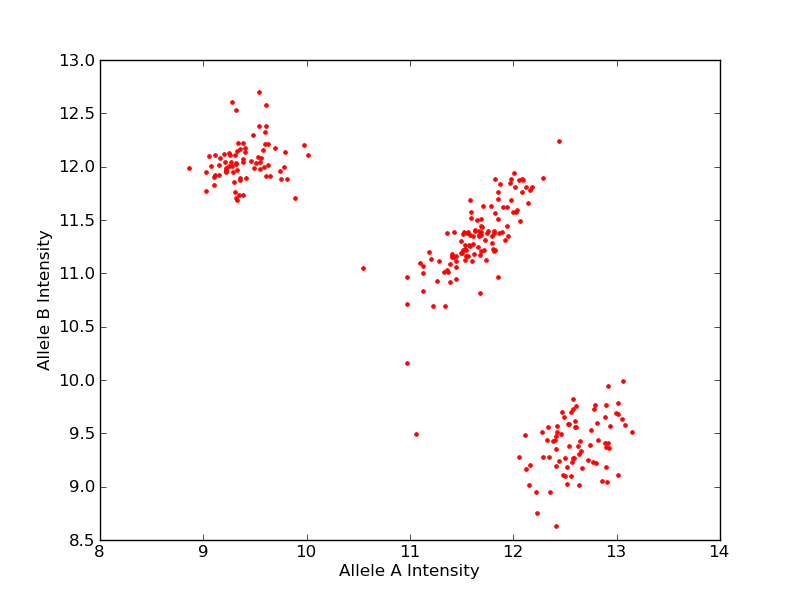
\includegraphics[scale=0.3]{data_figures/defined.png}
        \label{fig:dis_defined}
    }
    \subfigure[SNPs with less well defined genotype cluster]
    {
        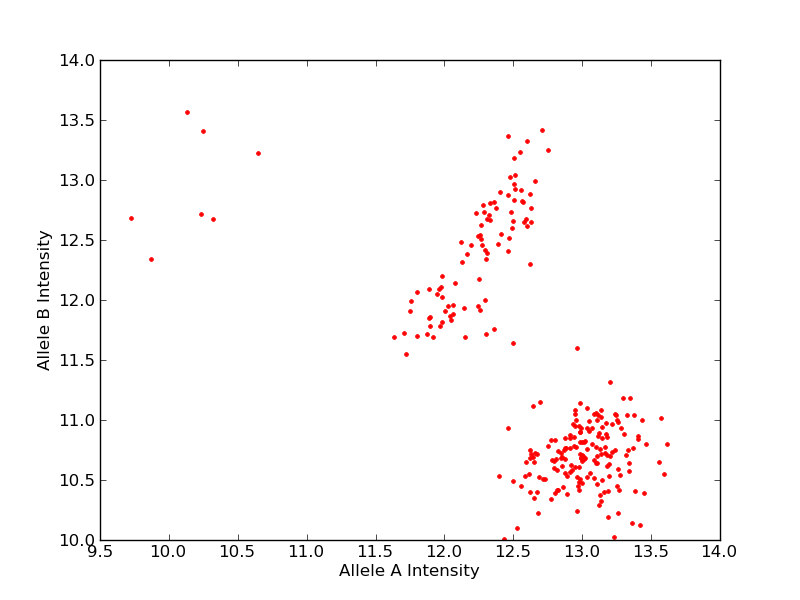
\includegraphics[scale=0.3]{data_figures/less_defined.png}
        \label{fig:dis_notdefined}
    }
    \caption{Genotype clusters for SNPs with different minor allele frequency}
    \label{fig:sample_subfigures}
\end{figure}

\par
Figure~\ref{fig:data_mafdist} shows the distribution of minor allele
frequencies of the SNPs selected for this project.
Most of the SNPs used in this project have moderate minor allele frequencies.
\begin{figure}[H]
    \centering
    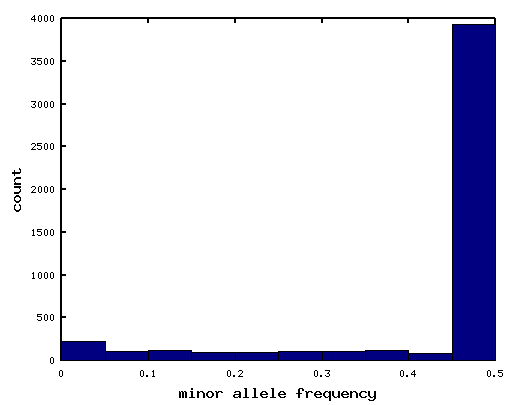
\includegraphics[scale=0.5]
    {data_figures/data_mafdist.png}
    \caption{MAF distribution for the selected SNPs used in this project}
    \label{fig:data_mafdist}
\end{figure}
%-----------------------------------------------------------------------------

%-----------------------------------------------------------------------------
% result
\section{Result}

\subsection{Implementation}

\par
The SoCal algorithm is implemented in Matlab with heavy use of CVX, which uses
interior method to solve conic programming problems.

\par
In general, the conic programming problems in this project can be solved in 
$O(\sqrt{v}log{{1}\over{\epsilon}})$ iterations, with each iteration
consisting of a damped Newton step \cite{glineur1998}.
The $v$ in the notation refers to the $v$-self-concordant barrier of the domain
of the conic programming problem, and $\epsilon$ the accuracy of the 
result \cite{glineur1998}.

\subsection{Training and validation}

\par
For each SNP, $33\%$ of individual samples data is randomly selected to train
the genotype caller to find the decision regions for each SNP.
And the rest $67\%$ of the data is used to validate the caller.
Three different methods for constructing ellipsoids, MAXSEP, MINVOL, and COMB
are tested on the dataset.
For COMB, $\beta_{1}$ is set to 1, $\beta_{2}$ is set 10, and $\beta_{3}$
is set to 100.
The parameters are meant to punish outlier effect.
Their performance is compared in the next section.

\subsection{Performance comparison}

Table~\ref{table:result_perfcmp} summarizes the performance of each method.
It's clear that although the COMB method is slower, it's much more accurate
than MAXSEP and MINVOL.
And after finding the elliptical decision regions, future genotype calls can be
done in linear time.
\begin{table}[H]
\centering
\begin{tabular}{|p{1.5cm}|p{1.5cm}|p{1.5cm}|p{1.5cm}|p{1.5cm}|p{1.5cm}|}
    \hline
    Method  & Accuracy (\%) & Training time (sec/SNP)
    & Calling time (sec/SNP) & Total training time (h)
    & Total calling time (sec)\\ \hline
    MINVOL  & 41.1          & 1.68 & 0.0 & 2.34 & 0.27 \\ \hline
    MAXSEP  & 72.7          & 1.43 & 0.0 & 1.98 & 0.33 \\ \hline  
    COMB    & 97.5          & 2.58 & 0.0 & 3.59 & 0.41 \\ \hline
\end{tabular}
\caption{Performance comparison for three different methods. K-means
algorithm was tested in a previous project.
The accuracy was 88.7\%, and it took about 5 seconds per SNP.
SoCal demonstrates that it's possible to use little
reference genotype call to achieve high genotype calling accuracy.}
\label{table:result_perfcmp}
\end{table}

\par
Figure~\ref{fig:method_classification} shows an example of the elliptical
decision regions found by SoCal for the three genotypes using the COMB method. 
\begin{figure}[H]
    \centering
    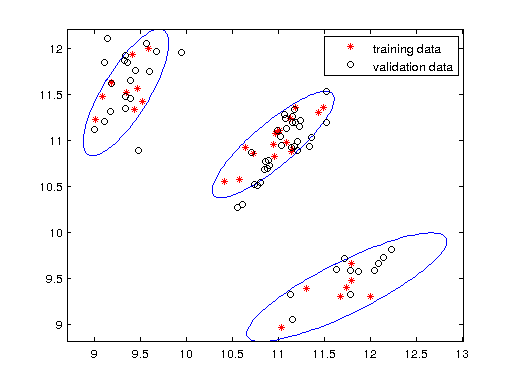
\includegraphics[scale=0.75]
    {result_figures/result_classification.png}
    \caption{Decision regions found by SoCal for all the
    three genotypes for SNP\_A-1641748}
    \label{fig:method_classification}
\end{figure}

\par
Figure~\ref{fig:result_mafacc} shows that the COMB method performs well even
for SNPs with low frequency, and is much better than the MINVOL and MAXSEP
methods.
This is because COMB takes into consideration three different objectives:
separation ratio, ellipsoid volume, and controlling outliers, where as the
other two methods only consider a single objective.
Therefore, COMB generalizes well even if the amount of data is limited.
But the other two methods tend to overfit the data.
\begin{figure}[H]
    \centering
    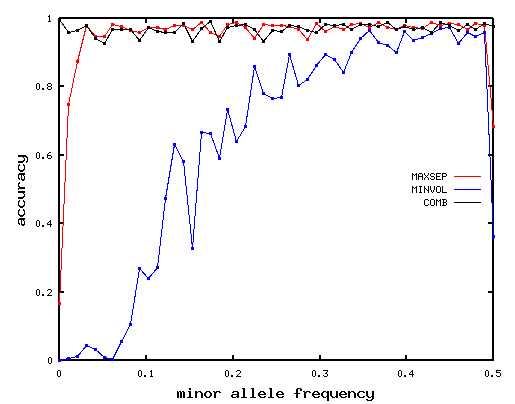
\includegraphics[scale=0.6]
    {result_figures/result_mafacc.png}
    \caption{Genotype calling accuracy for SNPs with different minor
             allele frequencies for MAXSEP, MINVOL, and COMB}
    \label{fig:result_mafacc}
\end{figure}
%-----------------------------------------------------------------------------

%-----------------------------------------------------------------------------
% discussion
\section{Discussion}

\par
SoCal demonstrates the possibility of using ellipsoids as decision
regions for classifying SNPs into genotypes.
In experiments involving HapMap data, SoCal is able to achieve $97.5\%$
genotype calling accuracy using only a small portion of reference genotype
calls.

\par
SoCal is different from many other genotype calling algorithms in different
aspects.
First, SoCal is a supervised genotype caller that uses reference genotype calls
to form decisions regions and then call genotypes for future SNPs.
Second, SoCal is efficient - the problem of finding separating ellipsoids
can be formulated as a conic programming problem and solved in polynomial time,
and is guaranteed to find a global optimum.
Third, the decision regions of SoCal can be used repeatedly.
Once the decision regions of a SNP for a particular SNP array are found,
future genotype calls can repeatedly use these regions without having to
first train a genotype caller.

\par
SoCal can be improved and extended in many ways.
First, for a SNP with low minor allele frequencies, the ellipsoid learned 
directly from one genotype may not be the best ellipsoid for classification
because of limited amount of data.
Instead, one can use the ellipsoids learned for other genotypes, which have
more data, to infer the ellipsoid for the genotype with relatively less data.
Second, SoCal can be extended to detect copy number variations in samples.
Individual samples with copy number variations may have extra A's or B's at
a SNP location. And if one plots the allele intensities $(I_A,I_B)$ for these
individuals, these data point will appear as outliers.
SoCal can use the ellipsoids learned from reference genotype calls to detect
outliers and then call copy number variations accordingly.

\par
In summary, SoCal is an efficient and accurate genotype caller for Affymetrix
SNP arrays. It can also be extended and improved to have more and
better functionalities.
%-----------------------------------------------------------------------------


%-----------------------------------------------------------------------------
% references
\begin{thebibliography}{9}
\bibitem{rho2010}
Rho, S. W., Abell, G. C., Kim, K., Nam, Y., \& Bae, J. (2010).
Comparing microarrays and next-generation sequencing technologies for microbial
ecology research. Trends in Biotechnology, 28, 291-299.
\bibitem{norlen2008}
Norl\'{e}n, H., Pettersson, E., Ahmadian, A., Lundeberg, J., \& Sundberg, R.
(2008). Classification of SNP genotypes by a Gaussian mixture model in
competitive enzymatic assays.
Mathematical Statistics Stockholm University Research Report, 3, 1-26.
\bibitem{lin2008}
Lin, Y., Tseng, G. C., Cheong, S. Y., Bean, L. J., Sherman, S. L., \&
Feingold, E. (2008). Smarter clustering methods for SNP genotype calling.
Bioinformatics, 24, 2665-2671.
\bibitem{wu1983}
Wu, C. F. (1983). On the Convergence Properties of the EM Algorithm.
The Annals of Statistics, 11, 95-103.
\bibitem{rabbee2005}
Rabbee, N., \& Speed, T. P. (2005).
A genotype calling algorithm for affymetrix SNP arrays.
Bioinformatics, 22, 7-12.
\bibitem{zhou2014}
Zhou, X., \& Stephens, M. (2014).
Efficient multivariate linear mixed model algorithms for genome-wide
association studies.
Nature Methods, 11, 407-409.
\bibitem{glineur1998}
Glineur F. (1998). Pattern separation via ellipsoids and conic programming.
(MS Thesis). Faculté Polytechnique de Mons, Mons, Belgium.
\end{thebibliography}
%-----------------------------------------------------------------------------

\end{document}
%-----------------------------------------------------------------------------
